% v3; 27 figures in DOCX order; genuine vector PDFs; TikZ masters preserved.
\begin{figure}[htbp]
\centering
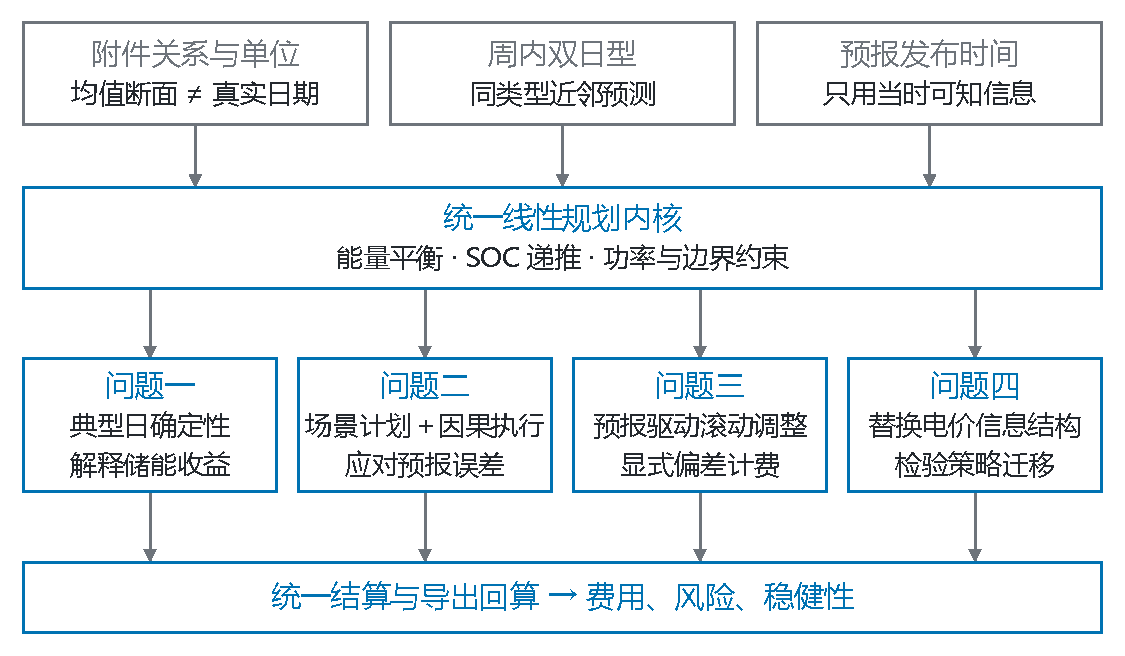
\includegraphics[width=155.44mm,keepaspectratio]{figures/fig_roadmap.pdf}
\caption{全文技术路线}
\label{fig:fig_roadmap}
\end{figure}

\begin{figure}[htbp]
\centering
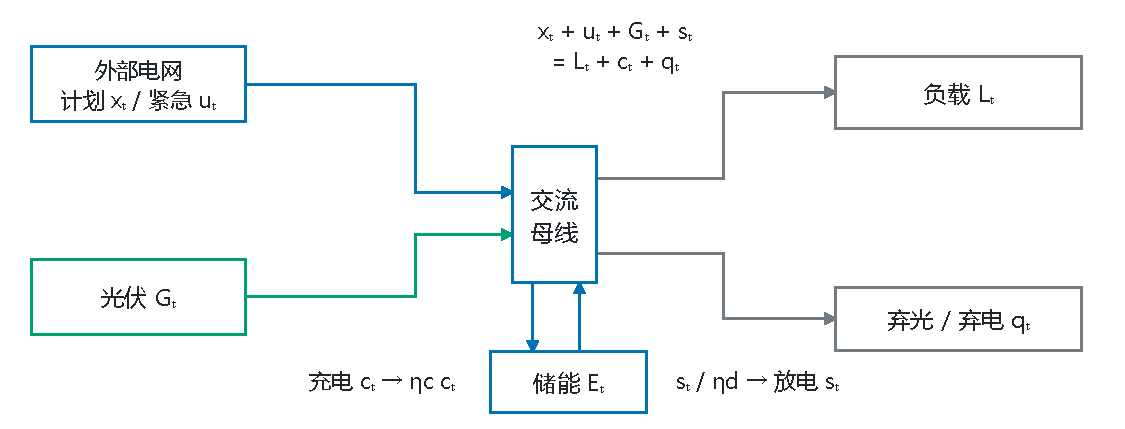
\includegraphics[width=150.00mm,keepaspectratio]{figures/fig_energy_flow.pdf}
\caption{交流母线能量流与储能效率作用位置}
\label{fig:fig_energy_flow}
\end{figure}

\begin{figure}[htbp]
\centering
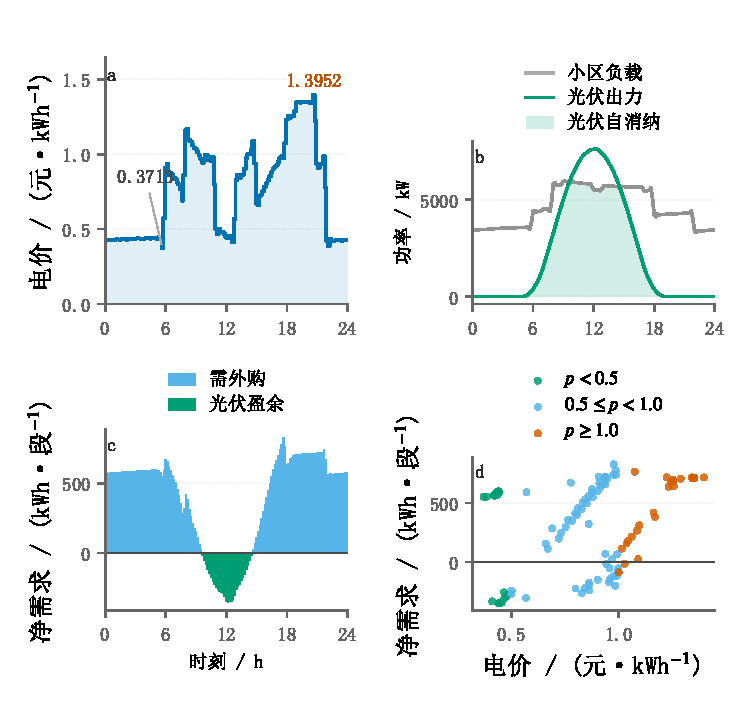
\includegraphics[width=116.69mm,keepaspectratio]{figures/fig_att1_profile.pdf}
\caption{附件一平均日断面}
\label{fig:fig_att1_profile}
\end{figure}

\begin{figure}[htbp]
\centering
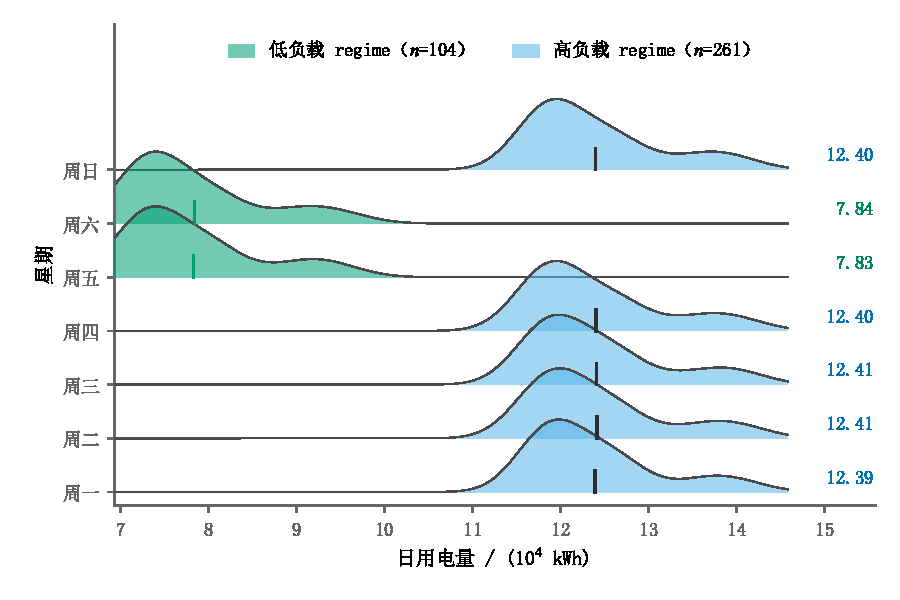
\includegraphics[width=146.25mm,keepaspectratio]{figures/fig_load_regime_ridgeline.pdf}
\caption{日用电量按星期分布}
\label{fig:fig_load_regime_ridgeline}
\end{figure}

\begin{figure}[htbp]
\centering
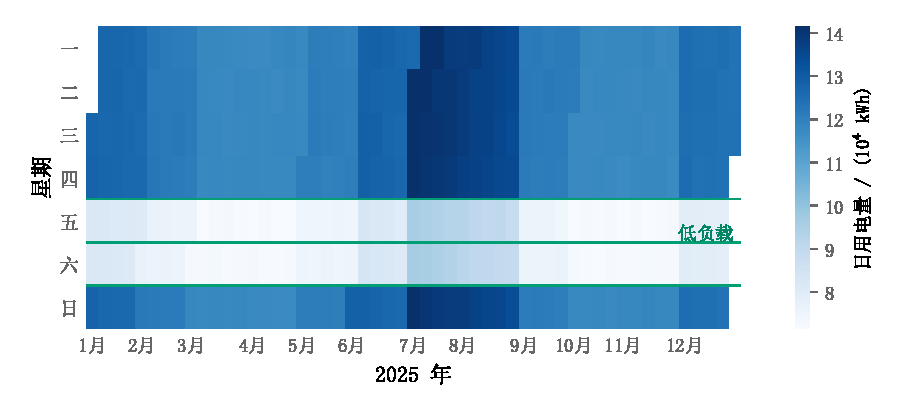
\includegraphics[width=146.25mm,keepaspectratio]{figures/fig_load_calendar.pdf}
\caption{全年日用电量日历热图}
\label{fig:fig_load_calendar}
\end{figure}

\begin{figure}[htbp]
\centering
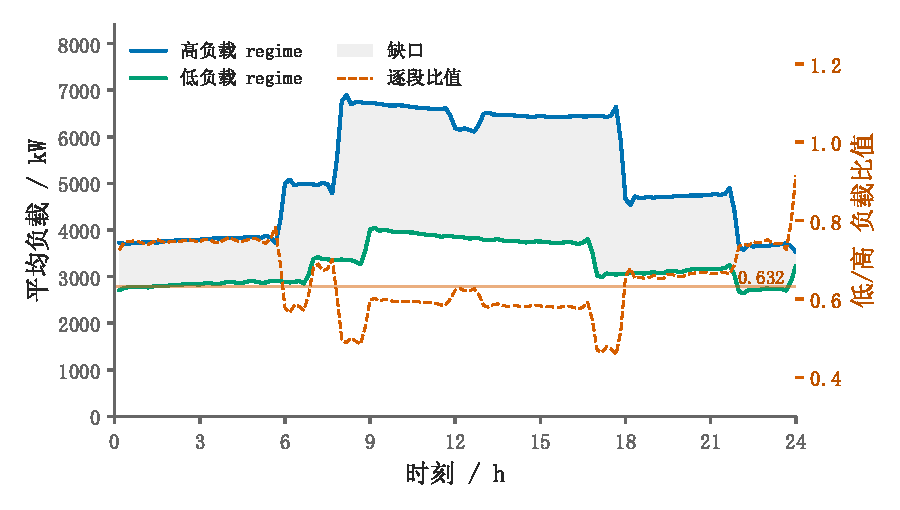
\includegraphics[width=146.25mm,keepaspectratio]{figures/fig_regime_shape.pdf}
\caption{两日型日内负载形状}
\label{fig:fig_regime_shape}
\end{figure}

\begin{figure}[htbp]
\centering
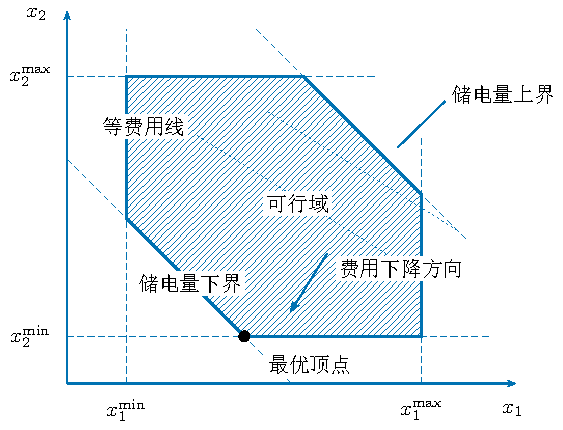
\includegraphics[width=156.00mm,keepaspectratio]{figures/tikz_feasible_q1.pdf}
\caption{相邻两段可行域示意}
\label{fig:tikz_feasible_q1}
\end{figure}

\begin{figure}[htbp]
\centering
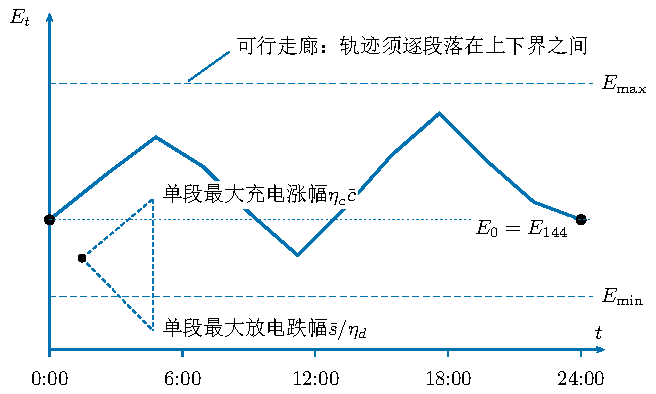
\includegraphics[width=156.00mm,keepaspectratio]{figures/tikz_soc_corridor.pdf}
\caption{储电量可行走廊示意}
\label{fig:tikz_soc_corridor}
\end{figure}

\begin{figure}[htbp]
\centering
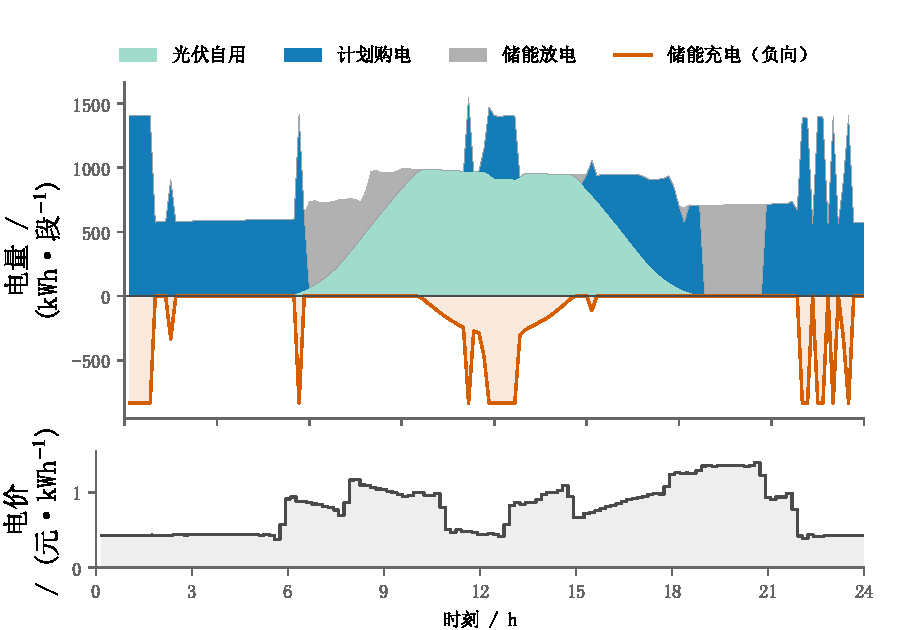
\includegraphics[width=146.25mm,keepaspectratio]{figures/fig_q1_dispatch_stack.pdf}
\caption{问题一最优调度构成}
\label{fig:fig_q1_dispatch_stack}
\end{figure}

\begin{figure}[htbp]
\centering
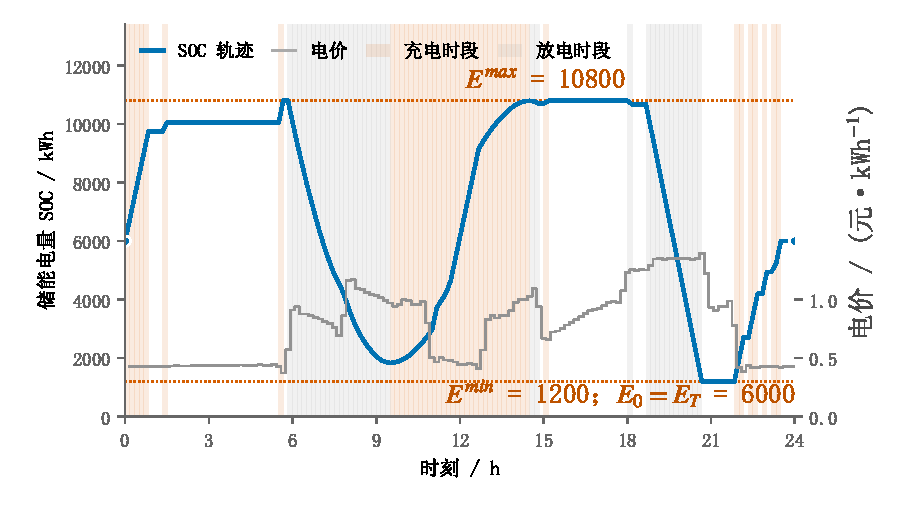
\includegraphics[width=146.25mm,keepaspectratio]{figures/fig_q1_soc_price.pdf}
\caption{问题一储电量与电价相位}
\label{fig:fig_q1_soc_price}
\end{figure}

\begin{figure}[htbp]
\centering
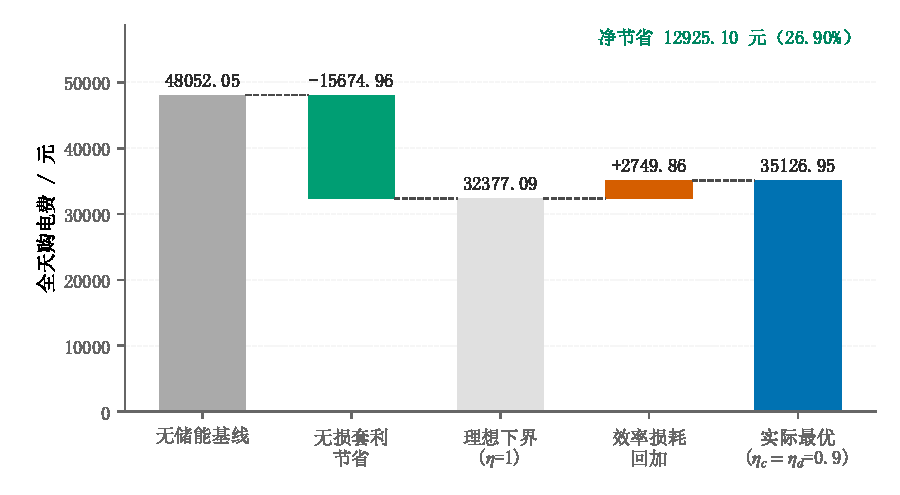
\includegraphics[width=146.25mm,keepaspectratio]{figures/fig_q1_savings_waterfall.pdf}
\caption{问题一费用瀑布分解}
\label{fig:fig_q1_savings_waterfall}
\end{figure}

\begin{figure}[htbp]
\centering
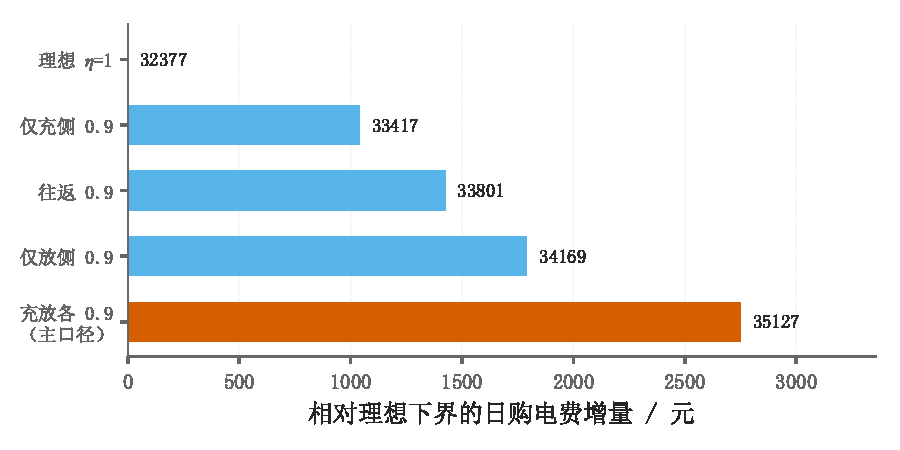
\includegraphics[width=146.25mm,keepaspectratio]{figures/fig_eta_sensitivity.pdf}
\caption{效率读法灵敏度}
\label{fig:fig_eta_sensitivity}
\end{figure}

\begin{figure}[htbp]
\centering
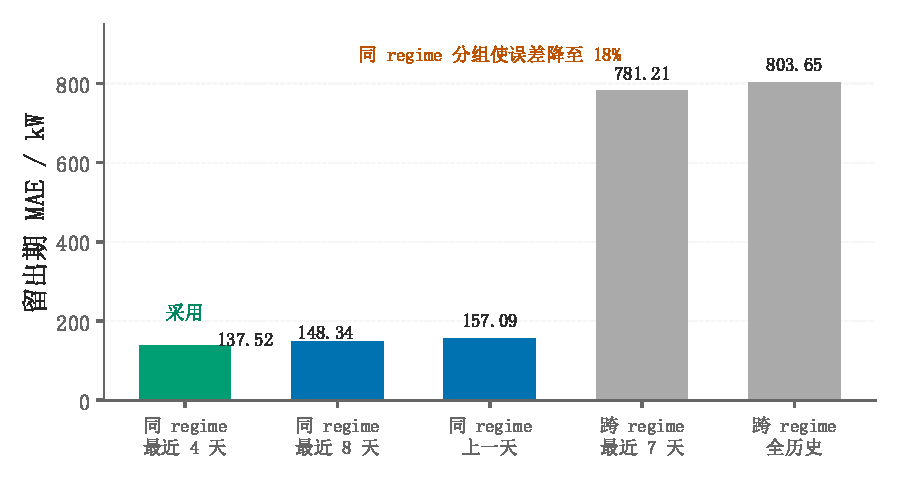
\includegraphics[width=146.25mm,keepaspectratio]{figures/fig_predictor_mae_bar.pdf}
\caption{负载预测器误差对比}
\label{fig:fig_predictor_mae_bar}
\end{figure}

\begin{figure}[htbp]
\centering
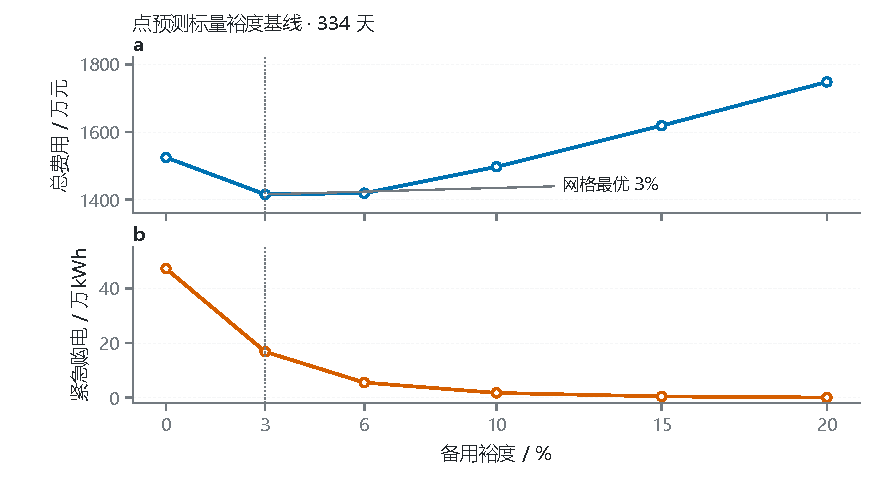
\includegraphics[width=146.25mm,keepaspectratio]{figures/fig_q2_margin_ucurve.pdf}
\caption{点预测基线的裕度费用与风险权衡}
\label{fig:fig_q2_margin_ucurve}
\end{figure}

\begin{figure}[htbp]
\centering
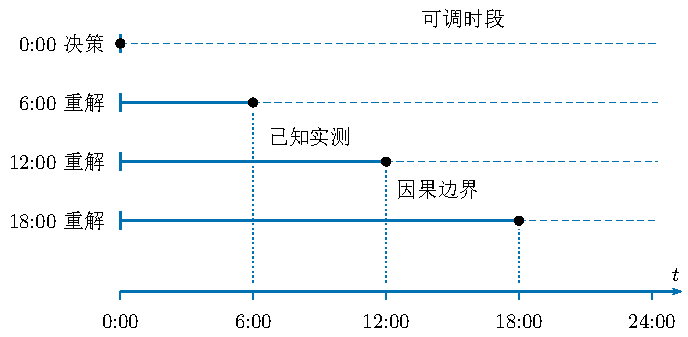
\includegraphics[width=156.00mm,keepaspectratio]{figures/tikz_info_set.pdf}
\caption{滚动决策信息集示意}
\label{fig:tikz_info_set}
\end{figure}

\begin{figure}[htbp]
\centering
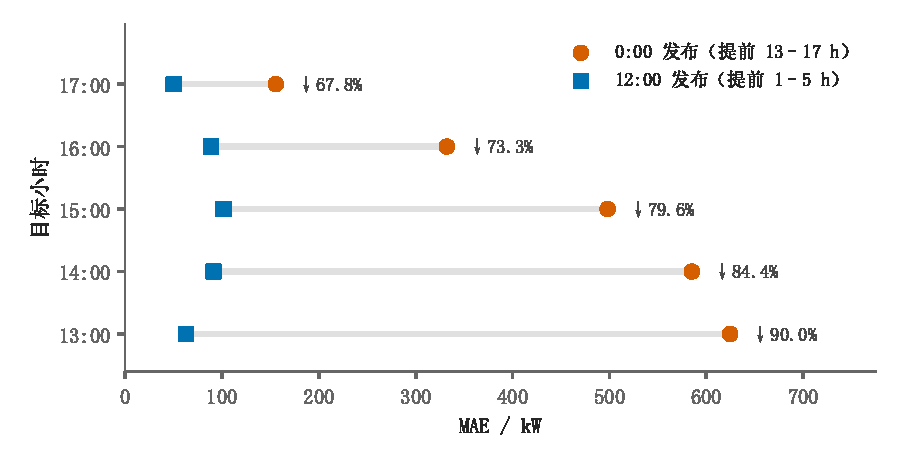
\includegraphics[width=146.25mm,keepaspectratio]{figures/fig_forecast_same_target.pdf}
\caption{同目标不同发布时刻预报}
\label{fig:fig_forecast_same_target}
\end{figure}

\begin{figure}[htbp]
\centering
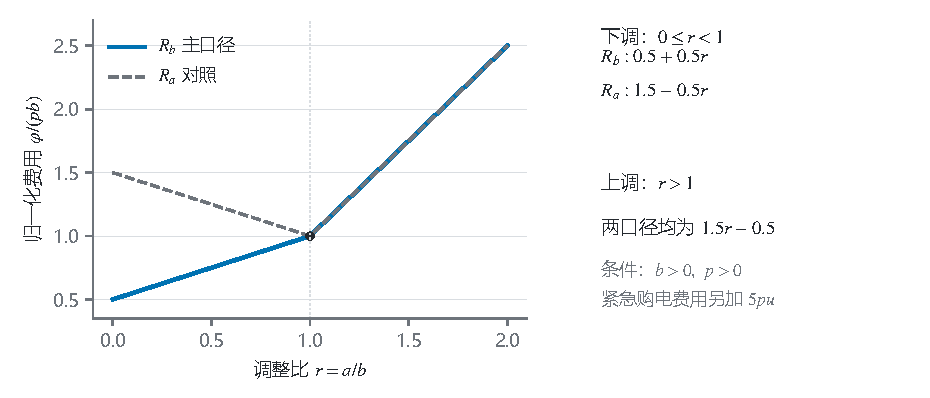
\includegraphics[width=150.00mm,keepaspectratio]{figures/fig_settlement_rule.pdf}
\caption{两种结算口径的归一化分段费用}
\label{fig:fig_settlement_rule}
\end{figure}

\begin{figure}[htbp]
\centering
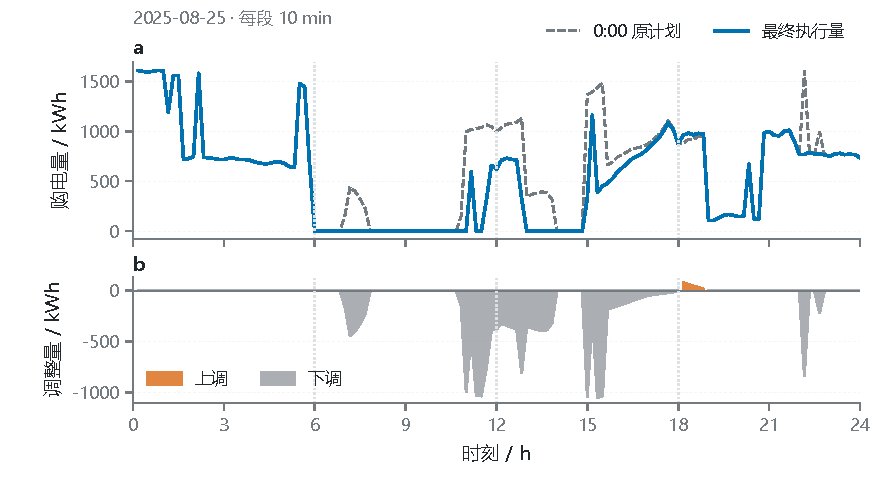
\includegraphics[width=155.59mm,keepaspectratio]{figures/fig_q3_rolling_timeline.pdf}
\caption{滚动决策结构与执行}
\label{fig:fig_q3_rolling_timeline}
\end{figure}

\begin{figure}[htbp]
\centering
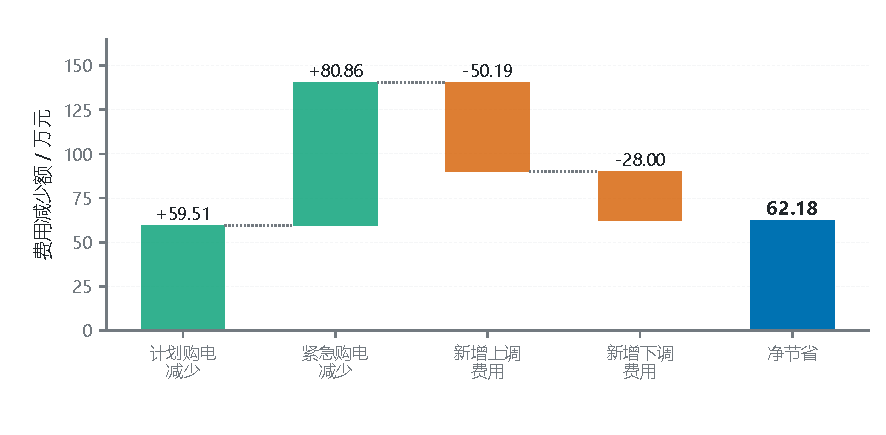
\includegraphics[width=146.25mm,keepaspectratio]{figures/fig_q3_cost_decomp.pdf}
\caption{问题三费用构成分解}
\label{fig:fig_q3_cost_decomp}
\end{figure}

\begin{figure}[htbp]
\centering
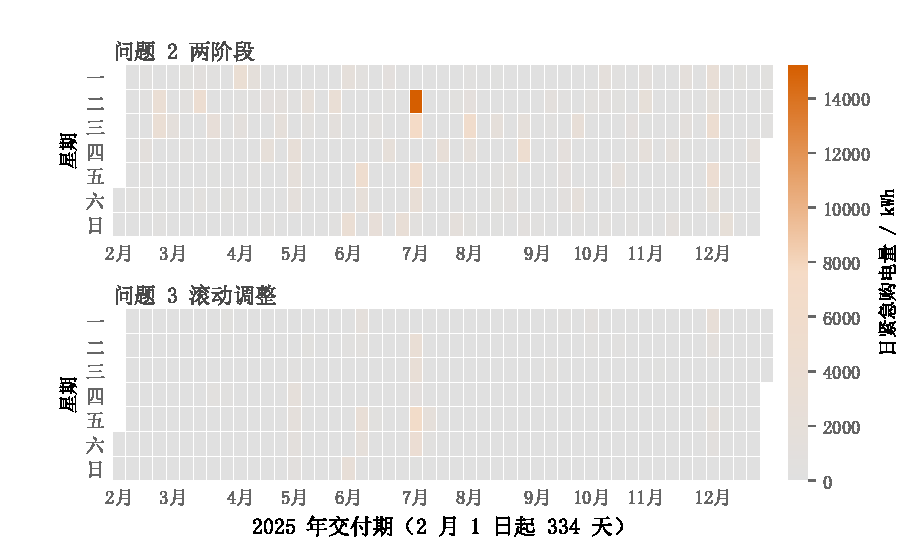
\includegraphics[width=146.25mm,keepaspectratio]{figures/fig_q2_emergency_calendar.pdf}
\caption{两方案紧急购电日历对比}
\label{fig:fig_q2_emergency_calendar}
\end{figure}

\begin{figure}[htbp]
\centering
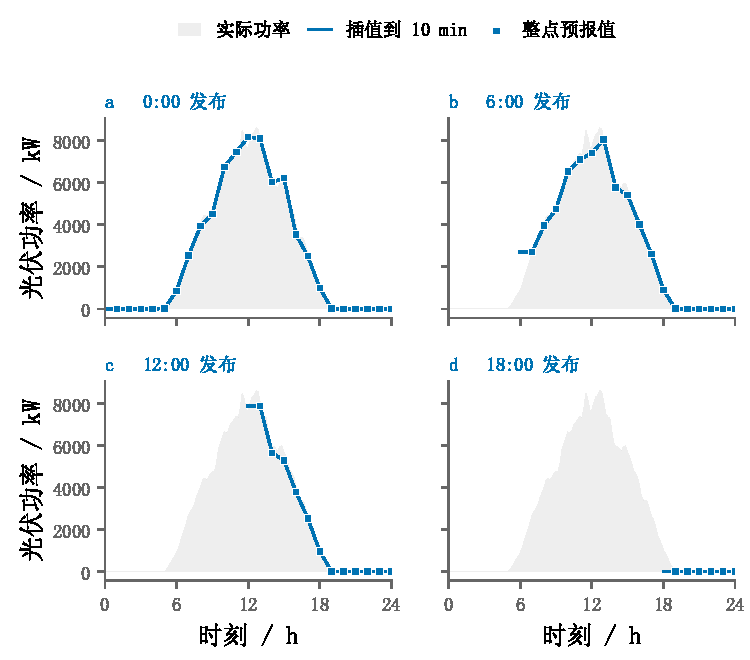
\includegraphics[width=110.80mm,keepaspectratio]{figures/fig_q3_interp_check.pdf}
\caption{预报插值一致性核查}
\label{fig:fig_q3_interp_check}
\end{figure}

\begin{figure}[htbp]
\centering
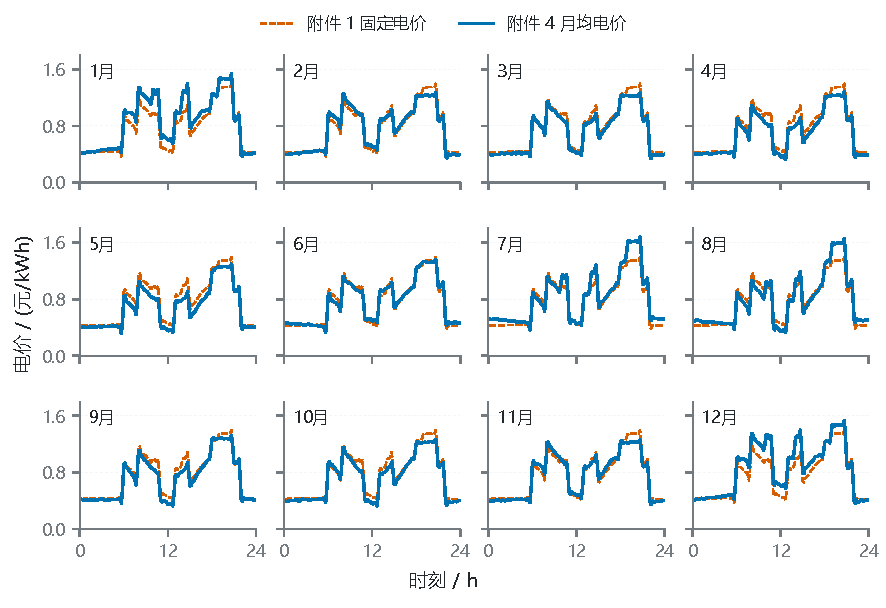
\includegraphics[width=146.25mm,keepaspectratio]{figures/fig_q4_price_ridgeline.pdf}
\caption{波动电价逐月日内曲线}
\label{fig:fig_q4_price_ridgeline}
\end{figure}

\begin{figure}[htbp]
\centering
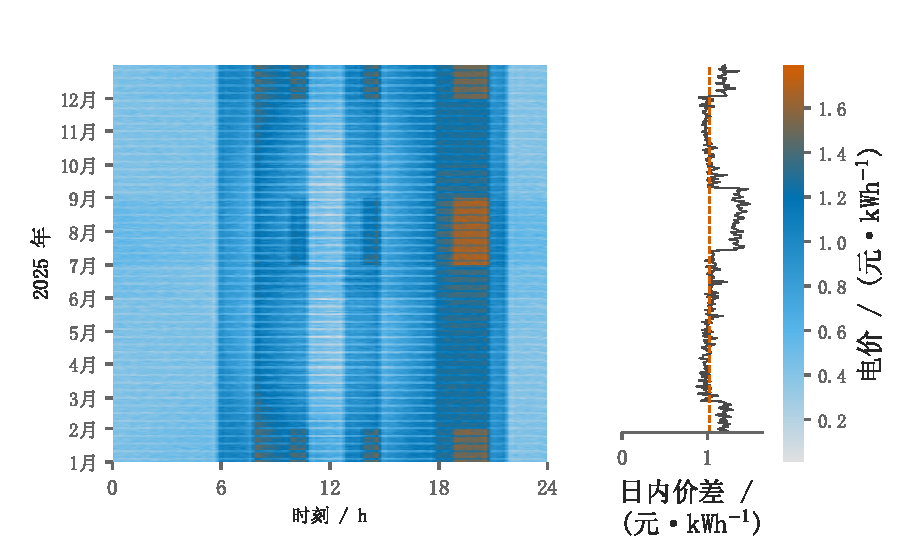
\includegraphics[width=146.25mm,keepaspectratio]{figures/fig_q4_price_hovmoller.pdf}
\caption{波动电价日期时刻热图}
\label{fig:fig_q4_price_hovmoller}
\end{figure}

\begin{figure}[htbp]
\centering
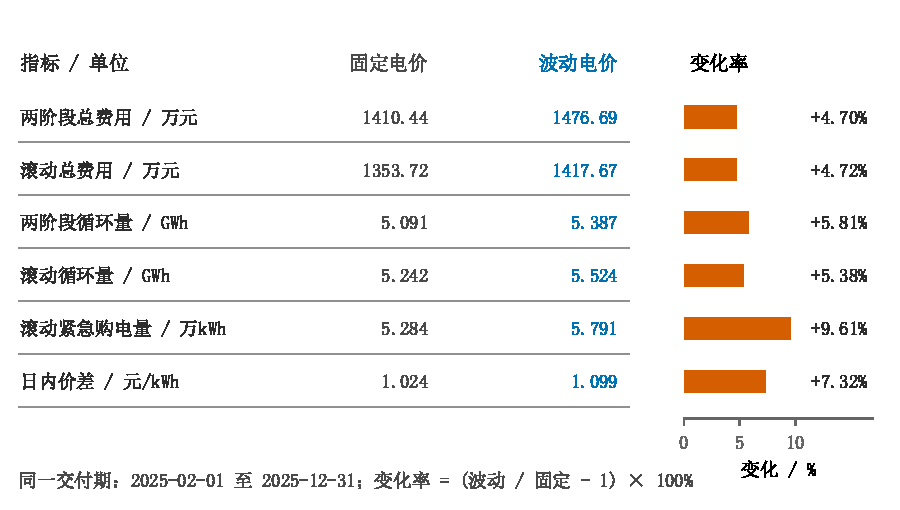
\includegraphics[width=146.25mm,keepaspectratio]{figures/fig_q4_fixed_vs_vol.pdf}
\caption{固定与波动电价指标对照}
\label{fig:fig_q4_fixed_vs_vol}
\end{figure}

\begin{figure}[htbp]
\centering
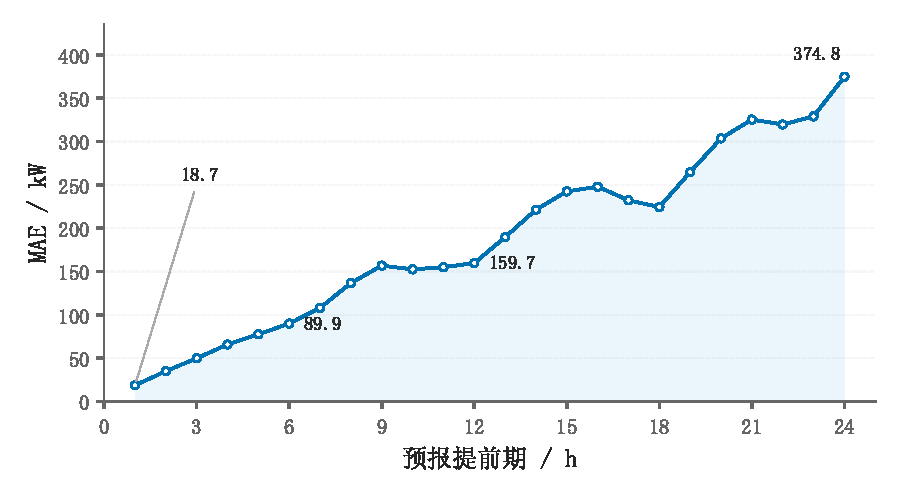
\includegraphics[width=146.25mm,keepaspectratio]{figures/fig_forecast_decay.pdf}
\caption{光伏预报误差随提前期变化}
\label{fig:fig_forecast_decay}
\end{figure}

\begin{figure}[htbp]
\centering
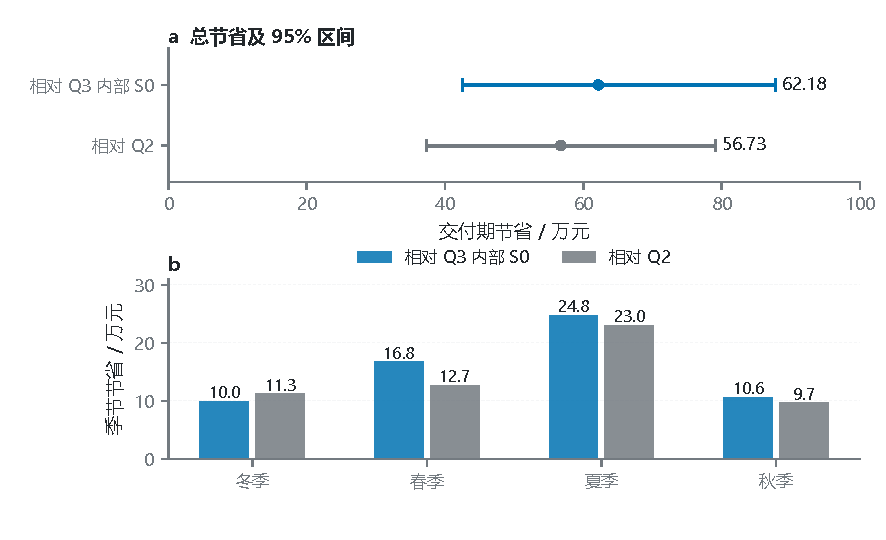
\includegraphics[width=150.00mm,keepaspectratio]{figures/fig_rolling_benefit_uncertainty.pdf}
\caption{滚动策略的配对收益区间与累计节省}
\label{fig:fig_rolling_benefit_uncertainty}
\end{figure}

\begin{figure}[htbp]
\centering
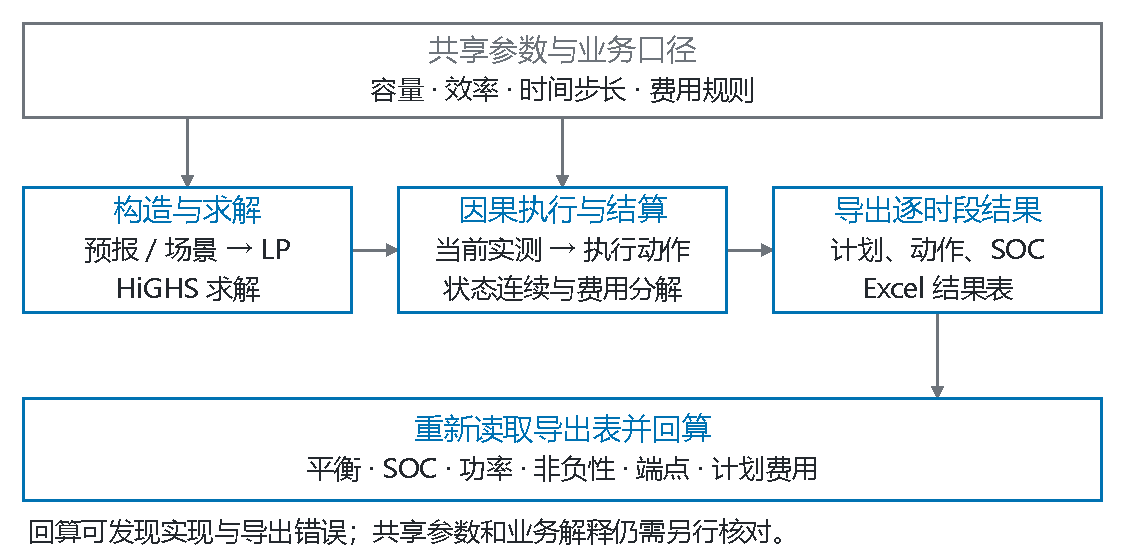
\includegraphics[width=155.36mm,keepaspectratio]{figures/fig_arch_solver.pdf}
\caption{求解程序模块依赖}
\label{fig:fig_arch_solver}
\end{figure}